\begingroup
\hyphenpenalty=10000
\exhyphenpenalty=10000
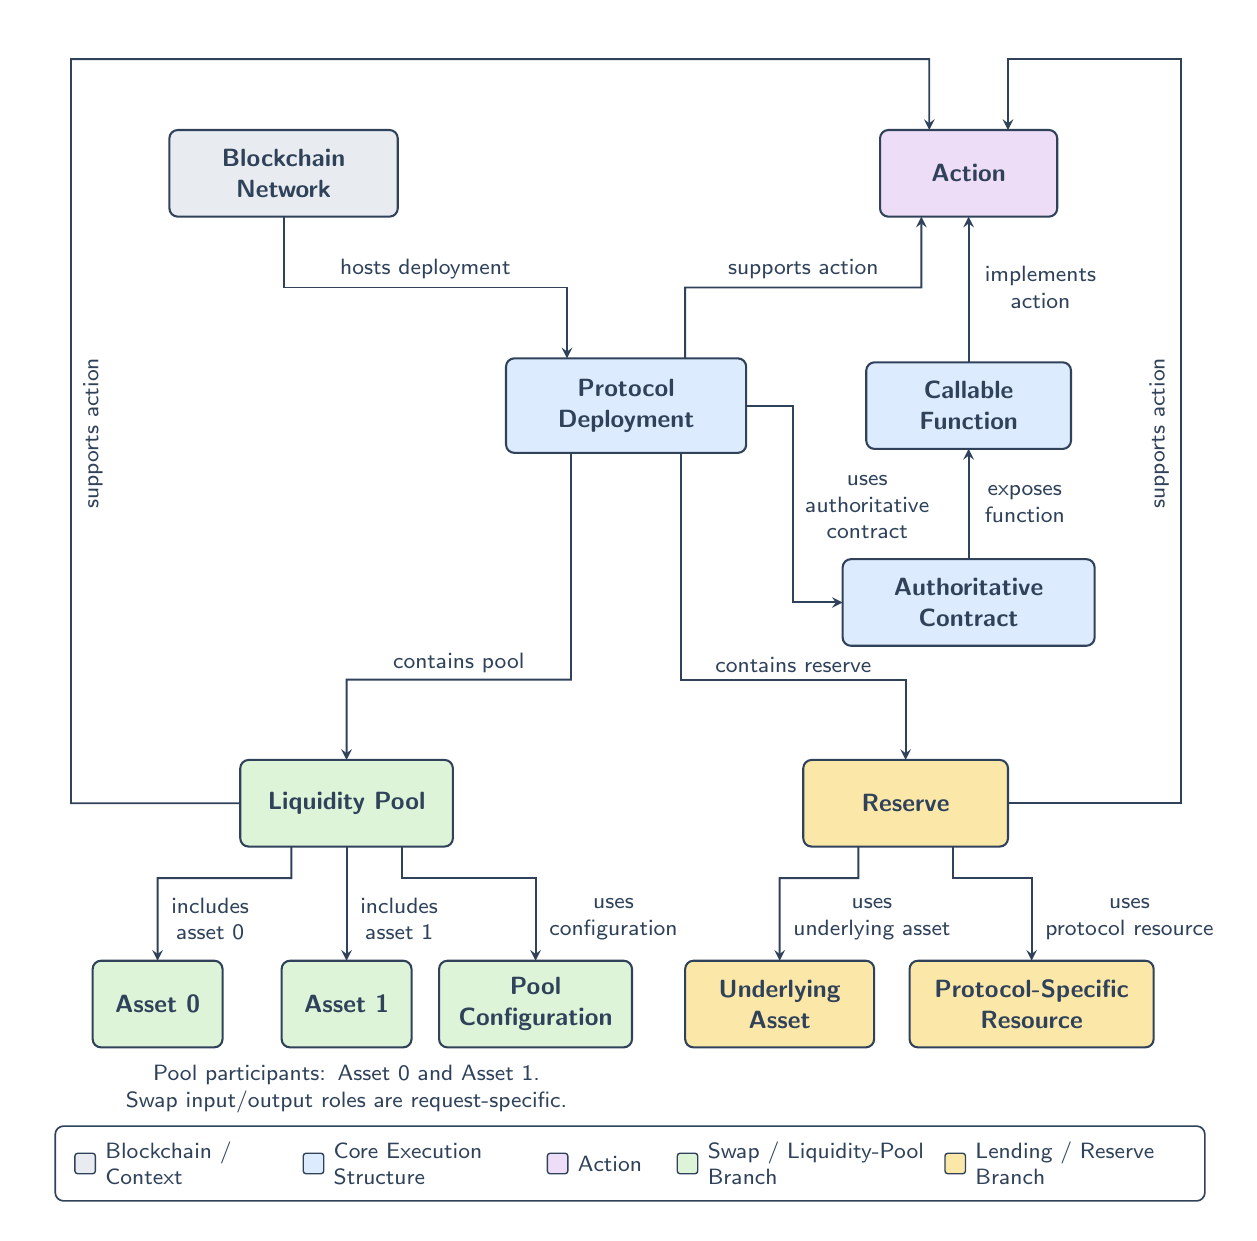
\begin{tikzpicture}[x=1cm,y=1cm,>=stealth]
\path[use as bounding box] (0,0) rectangle (15.25,15.05);

\definecolor{graphline}{HTML}{2F425A}
\definecolor{contextfill}{HTML}{E8ECF0}
\definecolor{corefill}{HTML}{DCEBFE}
\definecolor{actionfill}{HTML}{EEDDF6}
\definecolor{swapfill}{HTML}{DDF4D9}
\definecolor{lendfill}{HTML}{FBE8A9}

\tikzset{
  entity/.style={rectangle,rounded corners=3pt,draw=graphline,
    line width=0.75pt,align=center,text=graphline,
    inner xsep=4pt,inner ysep=4pt,outer sep=0pt,
    font=\sffamily\bfseries\fontsize{9.4}{11.2}\selectfont},
  relation/.style={->,draw=graphline,line width=0.70pt},
  relationlabel/.style={text=graphline,align=center,fill=white,
    inner sep=2pt,outer sep=0pt,
    font=\sffamily\fontsize{8.2}{9.6}\selectfont},
  note/.style={text=graphline,align=center,
    font=\sffamily\fontsize{8.1}{9.7}\selectfont},
  legendlabel/.style={text=graphline,anchor=west,inner sep=0pt,
    font=\sffamily\fontsize{8.0}{9.5}\selectfont}
}

% =========================================================
% Network, deployment and execution structure
% =========================================================
\node[entity,fill=contextfill,text width=2.50cm,
  minimum width=2.90cm,minimum height=1.10cm]
  (network) at (3.25,13.20) {Blockchain\\Network};
\node[entity,fill=actionfill,text width=1.95cm,
  minimum width=2.25cm,minimum height=1.10cm]
  (action) at (11.95,13.20) {Action};
\node[entity,fill=corefill,text width=2.65cm,
  minimum width=3.05cm,minimum height=1.20cm]
  (deployment) at (7.60,10.25) {Protocol\\Deployment};
\node[entity,fill=corefill,text width=2.20cm,
  minimum width=2.60cm,minimum height=1.10cm]
  (function) at (11.95,10.25) {Callable\\Function};
\node[entity,fill=corefill,text width=2.80cm,
  minimum width=3.20cm,minimum height=1.10cm]
  (contract) at (11.95,7.75) {Authoritative\\Contract};

% =========================================================
% Swap and lending branches: aligned parent and leaf rows
% =========================================================
\node[entity,fill=swapfill,text width=2.30cm,
  minimum width=2.70cm,minimum height=1.10cm]
  (pool) at (4.05,5.20) {Liquidity Pool};
\node[entity,fill=lendfill,text width=2.20cm,
  minimum width=2.60cm,minimum height=1.10cm]
  (reserve) at (11.15,5.20) {Reserve};

\node[entity,fill=swapfill,text width=1.35cm,
  minimum width=1.65cm,minimum height=1.10cm]
  (assetZero) at (1.65,2.65) {Asset 0};
\node[entity,fill=swapfill,text width=1.35cm,
  minimum width=1.65cm,minimum height=1.10cm]
  (assetOne) at (4.05,2.65) {Asset 1};
\node[entity,fill=swapfill,text width=2.15cm,
  minimum width=2.45cm,minimum height=1.10cm]
  (poolConfig) at (6.45,2.65) {Pool\\Configuration};
\node[entity,fill=lendfill,text width=2.00cm,
  minimum width=2.40cm,minimum height=1.10cm]
  (assetLend) at (9.55,2.65) {Underlying\\Asset};
\node[entity,fill=lendfill,text width=2.75cm,
  minimum width=3.10cm,minimum height=1.10cm]
  (resource) at (12.75,2.65) {Protocol-Specific\\Resource};

% =========================================================
% The two outer return paths enter Action through separate top ports.
\tikzset{edgecaption/.style={relationlabel,fill=none,inner sep=1pt}}
\draw[relation] (pool.west) -- (0.55,5.20) -- (0.55,14.65)
  -- (11.45,14.65) -- ([xshift=-0.50cm]action.north);
\draw[relation] (reserve.east) -- (14.65,5.20) -- (14.65,14.65)
  -- (12.45,14.65) -- ([xshift=0.50cm]action.north);
\node[edgecaption,rotate=90] at (0.83,9.90) {supports action};
\node[edgecaption,rotate=90] at (14.37,9.90) {supports action};

% Core execution structure.
\draw[relation] (network.south) -- (3.25,11.75)
  -- (6.85,11.75) -- ([xshift=-0.75cm]deployment.north);
\node[edgecaption,anchor=south] at (5.05,11.82) {hosts deployment};
\draw[relation] ([xshift=0.75cm]deployment.north) -- (8.35,11.75)
  -- (11.35,11.75) -- ([xshift=-0.60cm]action.south);
\node[edgecaption,anchor=south] at (9.85,11.82) {supports action};
\draw[relation] (function.north) -- (action.south);
\node[edgecaption,anchor=west] at (12.12,11.75) {implements\\action};
\draw[relation] (contract.north) -- (function.south);
\node[edgecaption,anchor=west] at (12.12,9.00) {exposes\\function};
\draw[relation] (deployment.east) -- (9.72,10.25)
  -- (9.72,7.75) -- (contract.west);
\node[edgecaption,anchor=west] at (9.84,8.96) {uses\\authoritative\\contract};

% Mirrored membership routes: separate departure ports, common bend height.
\draw[relation] ([xshift=-0.70cm]deployment.south) -- (6.90,6.77)
  -- (4.05,6.77) -- (pool.north);
\draw[relation] ([xshift=0.70cm]deployment.south) -- (8.30,6.77)
  -- (11.15,6.77) -- (reserve.north);
\node[edgecaption,anchor=south] at (5.475,6.82) {contains pool};
\node[edgecaption,anchor=south] at (9.725,6.82) {contains reserve};

% Each leaf has its own edge (no shared stem or ambiguous junction).
\draw[relation] ([xshift=-0.70cm]pool.south) -- (3.35,4.25)
  -- (1.65,4.25) -- (assetZero.north);
\draw[relation] (pool.south) -- (assetOne.north);
\draw[relation] ([xshift=0.70cm]pool.south) -- (4.75,4.25)
  -- (6.45,4.25) -- (poolConfig.north);
\draw[relation] ([xshift=-0.60cm]reserve.south) -- (10.55,4.25)
  -- (9.55,4.25) -- (assetLend.north);
\draw[relation] ([xshift=0.60cm]reserve.south) -- (11.75,4.25)
  -- (12.75,4.25) -- (resource.north);
\node[edgecaption,anchor=west] at (1.79,3.73) {includes\\asset 0};
\node[edgecaption,anchor=west] at (4.19,3.73) {includes\\asset 1};
\node[edgecaption,anchor=west] at (6.59,3.73) {uses\\configuration};
\node[edgecaption,anchor=west] at (9.69,3.73) {uses\\underlying asset};
\node[edgecaption,anchor=west] at (12.89,3.73) {uses\\protocol resource};

% Asset roles are request-specific, not additional graph entities.
\node[note,text width=7.00cm] at (4.05,1.57)
  {Pool participants: Asset 0 and Asset 1.\\
   Swap input/output roles are request-specific.};

% =========================================================
% One-row legend: conceptual roles, not approval or trust status
% =========================================================
\draw[draw=graphline,rounded corners=3pt,line width=0.6pt]
  (0.35,0.15) rectangle (14.95,1.10);
\foreach \GraphLegendX/\GraphLegendColour/\GraphLegendWidth/\GraphLegendText in {
  0.60/contextfill/2.35/{Blockchain /\\Context},
  3.50/corefill/2.55/{Core Execution\\Structure},
  6.60/actionfill/1.15/{Action},
  8.25/swapfill/2.75/{Swap / Liquidity-Pool\\Branch},
  11.65/lendfill/2.55/{Lending / Reserve\\Branch}}
{
  \draw[draw=graphline,fill=\GraphLegendColour,rounded corners=1pt,line width=0.5pt]
    (\GraphLegendX,0.495) rectangle ({\GraphLegendX+0.26},0.755);
  \node[legendlabel,text width=\GraphLegendWidth cm,align=left]
    at ({\GraphLegendX+0.38},0.625) {\GraphLegendText};
}
\end{tikzpicture}
\endgroup